\documentclass[11pt,a4paper]{article}

\usepackage[T1]{fontenc}
\usepackage[utf8]{inputenc}
\usepackage[provide=*,main=english]{babel}
\usepackage{lmodern}
\usepackage{microtype}
\usepackage{geometry}
\geometry{top=2.25cm,bottom=2.35cm,left=2.35cm,right=2.35cm}
\usepackage{amsmath,amssymb,amsthm,mathtools,bm}
\usepackage{graphicx}
\usepackage{booktabs,tabularx,array,multirow}
\usepackage{enumitem}
\usepackage{xcolor}
\usepackage{caption}
\usepackage{subcaption}
\usepackage{fancyhdr}
\usepackage{hyperref}
\usepackage[nameinlink,noabbrev]{cleveref}

\definecolor{deepblue}{RGB}{21,101,192}
\definecolor{deeporange}{RGB}{216,67,21}
\definecolor{softblue}{RGB}{232,242,252}
\definecolor{softgray}{RGB}{246,247,249}
\hypersetup{
  colorlinks=true,
  linkcolor=deepblue,
  citecolor=deepblue,
  urlcolor=deeporange,
  pdftitle={Spherical attention without an MLP: exact equilibria and cycles},
  pdfauthor={Anonymous submission}
}

\pagestyle{fancy}
\fancyhf{}
\fancyhead[L]{Spherical attention without an MLP}
\fancyhead[R]{Equilibria and cycles}
\fancyfoot[C]{\thepage}
\setlength{\headheight}{14.3pt}
\setlength{\parindent}{0pt}
\setlength{\parskip}{0.52em}
\setlength{\emergencystretch}{3em}
\setcounter{tocdepth}{1}
\setlist{nosep,leftmargin=*}

\newtheorem{theorem}{Theorem}[section]
\newtheorem{proposition}[theorem]{Proposition}
\newtheorem{lemma}[theorem]{Lemma}
\newtheorem{corollary}[theorem]{Corollary}
\theoremstyle{definition}
\newtheorem{definition}[theorem]{Definition}
\newtheorem{remark}[theorem]{Remark}

\newcommand{\sphere}{\mathbb S}
\newcommand{\R}{\mathbb R}
\newcommand{\diag}{\operatorname{diag}}
\newcommand{\Diag}{\operatorname{Diag}}
\newcommand{\rank}{\operatorname{rank}}
\newcommand{\softmax}{\operatorname{softmax}}
\newcommand{\e}{\mathrm e}
\newcommand{\T}{\mathsf T}
\newcommand{\one}{\bm 1}
\newcommand{\norm}[1]{\left\lVert #1\right\rVert}
\newcommand{\ip}[2]{\left\langle #1,#2\right\rangle}
\newcolumntype{Y}{>{\raggedright\arraybackslash}X}

\title{\textbf{Spherical Attention without an MLP:\\
Exact Equilibria, Multistability, and a Stable Internal Cycle}\\[0.5em]
\large A Reproducible Theoretical and Numerical Report}
\author{Anonymous submission}
\date{Version of August 16, 2026}

\begin{document}
\maketitle

\begin{abstract}
We study a stack of layers reduced to its attention mechanism: no MLP is present.
Each token is a unit-norm point, and each layer moves it and then renormalizes it.
We derive a necessary and sufficient condition, valid for any number of
tokens, any dimension, and arbitrary score and value matrices: at equilibrium, the
transported average seen by each token must be exactly parallel to that token. We give
the corresponding finite-layer condition, a reduction by groups, the exact
linearization, and, in the tied case $Q^{\T}K=V=V^{\T}$, a complete description in
terms of Gram matrices. This description contains consensus, two-sign partitions,
multi-vertex shapes, continuous families, and mixtures of eigendirections.

We distinguish finite-layer periodic orbits from periodic orbits of the continuous
flow. In the tied symmetric case, a strict Lyapunov function excludes every
nonconstant periodic orbit. For independent score and value matrices with
nonreciprocal value transport, attention alone admits a stable internal periodic
orbit with three tokens. Its return time is $9.12$ in normalized depth, and the two
transverse Lyapunov exponents are approximately $-0.457$ and $-0.459$. All 128 tested
perturbations return to the orbit. Across seven dyadic and nondyadic layer strengths,
the number of layers per revolution has log--log slope $1.012$, as required for
convergence to a finite-period continuous orbit. These computations establish
existence for one parameter set; they do not determine the frequency of periodic
orbits under a random matrix model.
\end{abstract}

\clearpage
\tableofcontents
\newpage

\section{Introduction}

A standard Transformer block combines attention, a residual connection,
normalization, and an MLP \cite{vaswani2017attention}. We study the subsystem obtained
by retaining attention, the residual connection, and spherical normalization. The
state consists of $n$ unit vectors in $\mathbb R^d$; the effective score matrix
$S=Q^{\mathsf T}K$ and value matrix $V$ are arbitrary unless symmetry is stated.

Particle descriptions of attention account for cluster formation
\cite{geshkovski2023clusters,geshkovski2025perspective}. Altafini classified four
equilibrium classes and derived stability conditions under symmetric $V$
\cite{altafini2025multistability}. Kuehn and Yoon studied the tied symmetric model
$Q^{\T}K=V=V^{\T}$ and obtained eigenspace-selection results
\cite{kuehnyoon2026spectral}. The results below address two complementary questions.
First, they characterize every stationary configuration for general $S,V$, with a
closed spectral--Gram formulation in the tied symmetric case. Second, they determine
which recurrent motions are compatible with the continuous-depth limit. The
equilibrium condition permits nonzero radial attention outputs, a distinction needed
to compare multi-vertex equilibria with Altafini's zero-output polygonal class. The
tied symmetric flow has a strict Lyapunov function. Untied score and value matrices
admit the explicit stable periodic orbit reported in \cref{sec:cycle-experiment}.

\section{The model, from one layer to continuous time}
\label{sec:model}

\subsection{Meaning of the symbols}

There are $n$ tokens. Token $i$ is a unit vector $x_i\in\R^d$, hence lies on the sphere
$\sphere^{d-1}$. Two matrices suffice:
\begin{itemize}
  \item $S=Q^{\T}K$ determines who attends to whom;
  \item $V$ determines which vector is actually transported.
\end{itemize}

The parameter $\beta\geq0$ controls the sharpness of the choice. At $\beta=0$, all
tokens receive equal weight. As $\beta$ increases, score differences matter more. For
a configuration $X=(x_1,\ldots,x_n)$, define
\begin{align}
 s_{ij}(X)&=x_i^{\T}Sx_j,\\
 a_{ij}(X)&=\frac{\exp(\beta s_{ij}(X))}
 {\sum_{k=1}^n\exp(\beta s_{ik}(X))},\\
 y_i(X)&=\sum_{j=1}^n a_{ij}(X)Vx_j. \label{eq:attention-output}
\end{align}
$a_{ij}$ is the weight assigned by $i$ to $j$, and $y_i$ is the sum received by $i$
after transport by $V$.

\subsection{A finite layer}

Without an MLP, the normalized residual layer is exactly
\begin{equation}
 x_i^+=\frac{x_i+h y_i(X)}{\norm{x_i+h y_i(X)}} ,
 \qquad i=1,\ldots,n,                                      \label{eq:finite-map}
\end{equation}
where $h>0$ is the layer strength. This spherical normalization is an idealized
version of RMSNorm \cite{zhang2019rmsnorm}.

\subsection{Many weak layers}

Write
\[
 P_x=I-xx^{\T}.
\]
$P_xz$ retains only the component of $z$ that changes the direction of $x$; the
component parallel to $x$ changes only its length and is removed by normalization.
Expanding \eqref{eq:finite-map} gives
\[
 x_i^+=x_i+hP_{x_i}y_i(X)+O(h^2).
\]
When the number of layers grows while $h$ decreases, the limit is
\begin{equation}
 \boxed{\quad \dot x_i=P_{x_i}y_i(X)
 =y_i(X)-\bigl(x_i^{\T}y_i(X)\bigr)x_i.\quad}              \label{eq:ode}
\end{equation}
The norm remains one because $x_i^{\T}\dot x_i=0$.

On the circle, write $x_i=(\cos\theta_i,\sin\theta_i)$ and
$t_i=(-\sin\theta_i,\cos\theta_i)$. The equation reduces to one scalar per token:
\begin{equation}
 \dot\theta_i=\sum_{j=1}^n a_{ij}(\theta)\,t_i^{\T}Vx_j.  \label{eq:circle}
\end{equation}
All cycle experiments in this report use this equation with three tokens.

\section{Equilibrium equations}
\label{sec:equilibria}

\begin{theorem}[Necessary and sufficient condition, general matrices]
\label{thm:general-equilibrium}
A configuration $X\in(\sphere^{d-1})^n$ is an equilibrium of \eqref{eq:ode} if and only
if, for every token $i$,
\begin{equation}
 \boxed{\quad y_i(X)=\lambda_i x_i,
 \qquad \lambda_i=x_i^{\T}y_i(X).\quad}                   \label{eq:parallel-condition}
\end{equation}
Equivalently, after removing the softmax denominator,
\begin{equation}
 \boxed{\quad
 \sum_{j=1}^n \e^{\beta x_i^{\T}Sx_j}
 \left[Vx_j-\bigl(x_i^{\T}Vx_j\bigr)x_i\right]=0,
 \qquad i=1,\ldots,n.\quad}                               \label{eq:final-equilibrium}
\end{equation}
\end{theorem}

\begin{proof}
The vector field is $P_{x_i}y_i$. It vanishes exactly when $y_i$ lies on the line
spanned by $x_i$. The collinearity coefficient is its inner product with $x_i$.
Finally, the softmax denominator is strictly positive, so multiplying by it or
removing it does not change the zero equality.
\end{proof}

The theorem permits $y_i\ne0$. Any radial output is removed by normalization, so a
multi-vertex equilibrium need not have zero attention output.

\subsection{Exact condition for a finite layer}

\begin{proposition}[Fixed point of one layer]
Assume $x_i+h y_i\neq0$. Layer \eqref{eq:finite-map} leaves $x_i$ unchanged if and only if
\begin{equation}
 P_{x_i}y_i=0
 \quad\text{and}\quad
 1+h\lambda_i>0,
 \qquad \lambda_i=x_i^{\T}y_i.                             \label{eq:finite-fixed}
\end{equation}
\end{proposition}

The first condition is the same as in continuous time. The second is specific to a
finite layer: if $1+h\lambda_i<0$, normalization sends the point to its antipode
$-x_i$; if $1+h\lambda_i=0$, it attempts to normalize the zero vector.

\subsection{Exact reduction when several tokens coincide}

Suppose the configuration contains only $q$ distinct positions
$w_1,\ldots,w_q$, repeated $r_1,\ldots,r_q$ times. Then
\eqref{eq:final-equilibrium} becomes the finite system
\begin{equation}
 \boxed{\quad
 \sum_{b=1}^q r_b\e^{\beta w_a^{\T}Sw_b}
 \left[Vw_b-\bigl(w_a^{\T}Vw_b\bigr)w_a\right]=0,
 \quad a=1,\ldots,q.\quad}                                \label{eq:cluster-reduction}
\end{equation}
This is not an approximation: only identical terms have been grouped. For a fixed
instance, \eqref{eq:cluster-reduction} gives an exhaustive procedure: enumerate the
partitions $r_1+\cdots+r_q=n$, solve the equations, and remove copies related by
permutation.

\subsection{Polygonal and clustering equilibria}
\label{sec:terminology}

Altafini \cite{altafini2025multistability} uses four names. The useful distinction is
summarized in \cref{tab:altafini-classes}.

\begin{table}[ht]
\centering
\caption{Altafini's four names, expressed using the sum $y_i$ from
\eqref{eq:attention-output}. The last two rows cover all noncollinear shapes.}
\label{tab:altafini-classes}
\begin{tabularx}{\textwidth}{@{}lXl@{}}
\toprule
Name & Configuration & Received-sum condition \\
\midrule
Consensus & all $x_i$ equal an eigendirection of $V$ & $y_i\parallel x_i$ \\
Bipolar consensus & each $x_i$ equals $u$ or $-u$, with $u$ an eigenvector & $y_i\parallel x_i$ \\
Polygonal & multiple directions and zero output & $y_i=0$ for every $i$ \\
Clustering & every other equilibrium, with or without coincident tokens & $y_i=\lambda_i x_i$, with at least one $\lambda_i\neq0$ \\
\bottomrule
\end{tabularx}
\end{table}

Thus, ``the points form a triangle'' is a visual description. ``Polygonal'' in the
sense of Altafini's theorem is a much narrower algebraic condition. A triangle whose
three outputs are nonzero and radial belongs to his fourth class. Instability of
zero-output equilibria says nothing about the stability of that triangle.

\section{Complete characterization in the tied symmetric case}
\label{sec:symmetric}

We now impose
\begin{equation}
 S=V=V^{\T}.                                                \label{eq:tied-symmetry}
\end{equation}
This is exactly the assumption of Kuehn--Yoon \cite{kuehnyoon2026spectral}. It is
stronger than Altafini's: Altafini assumes that $V$ is symmetric with a simple dominant
positive eigenvalue, but does not require $Q^{\T}K$ to be symmetric or equal to $V$.

Write the tokens as the rows of a matrix $X\in\R^{n\times d}$ and set
\[
 H=XVX^{\T},\qquad R=\exp_\circ(\beta H),
\]
where the exponential is applied entrywise. Define
\[
 M=\Diag\bigl(\diag(RH)\bigr).
\]

\begin{theorem}[Complete vector equation]
\label{thm:vector-complete}
Under \eqref{eq:tied-symmetry},
\begin{equation}
 \boxed{\quad X\text{ is an equilibrium}
 \iff RXV=MX,\qquad \diag(XX^{\T})=\one.\quad}              \label{eq:matrix-equilibrium}
\end{equation}
\end{theorem}

This formula is already necessary and sufficient. The next one removes rotations that
do not change the problem.

\begin{theorem}[Spectral description by Gram matrices]
\label{thm:spectral-gram}
Let $\lambda_1^\star,\ldots,\lambda_s^\star$ be the distinct eigenvalues of $V$, with
multiplicities $m_1,\ldots,m_s$. Write the component of $X$ in each eigenspace as
$C_\alpha\in\R^{n\times m_\alpha}$ and set $G_\alpha=C_\alpha C_\alpha^{\T}$.
Modulo internal rotations within eigenspaces, the equilibria are exactly the families
$(G_\alpha)$ satisfying
\begin{equation}
\boxed{
\begin{aligned}
 &G_\alpha\succeq0,\qquad \rank G_\alpha\le m_\alpha,\\
 &\sum_{\alpha=1}^s\diag G_\alpha=\one,\\
 &H=\sum_{\alpha=1}^s\lambda_\alpha^\star G_\alpha,
 \qquad R=\exp_\circ(\beta H),\\
 &M=\Diag\bigl(\diag(RH)\bigr),\\
 &(\lambda_\alpha^\star R-M)G_\alpha=0,
 \qquad \alpha=1,\ldots,s.
\end{aligned}}                                             \label{eq:spectral-gram}
\end{equation}
\end{theorem}

The proof in \cref{app:proofs} only projects \eqref{eq:matrix-equilibrium} onto each
eigenspace and factors the matrices $G_\alpha$. System \eqref{eq:spectral-gram} is a
complete characterization, not a preselected list of shapes.

\subsection{Families implied by the characterization}

\Cref{tab:families} lists the branches that exist without numerically solving a
particular instance.

\begin{table}[ht]
\centering
\caption{Exact families without an MLP under the tied symmetric assumption.}
\label{tab:families}
\begin{tabularx}{\textwidth}{@{}lX@{}}
\toprule
Situation & Equilibria or families guaranteed immediately \\
\midrule
$V=0$ & every configuration in $(\sphere^{d-1})^n$ \\
One token & all unit spheres contained in eigenspaces of $V$ \\
Consensus & $x_1=\cdots=x_n=u$ for every unit eigendirection $u$ \\
One eigenline & every sign pattern $x_i\in\{u,-u\}$ \\
Kernel of $V$ & every configuration contained in $\ker V$; mixed additions are possible if the active output vanishes \\
One repeated eigenspace & regular simplices, regular polygons, hypercubes, and other symmetric orbits, with compatible multiplicities \\
Several eigenspaces & mixed symmetric or asymmetric branches, solved by \eqref{eq:spectral-gram} or \eqref{eq:cluster-reduction} \\
\bottomrule
\end{tabularx}
\end{table}

There is therefore no finite list valid for every $n,d,V$: if $V=0$, every point is
an equilibrium; if an eigenvalue is repeated, continuous families appear. The proper
meaning of ``all equilibria'' is the constructive condition \eqref{eq:spectral-gram}.

\subsection{Fully explicit classification at \texorpdfstring{$\beta=0$}{beta = 0}}

At $\beta=0$, all weights equal $1/n$. Set
\[
 z=V\sum_{j=1}^n x_j.
\]

\begin{theorem}[All equilibria under uniform attention]
\label{thm:beta-zero}
For an arbitrary matrix $V$, a configuration is an equilibrium if and only if one of
the following two cases holds:
\begin{enumerate}
  \item $z=0$; every configuration satisfying $V\sum_jx_j=0$ is admissible;
  \item $z\neq0$; all tokens equal $u$ or $-u$, their signed sum is nonzero, and $u$
  is a real eigenvector of $V$ associated with a nonzero eigenvalue.
\end{enumerate}
\end{theorem}

This classification displays both the richness and fragility of the uniform case. With
a symmetric matrix, it is an energy dynamics. With a nonsymmetric matrix, a rotation
can persist even though the weights never change.

\subsection{An exact three-group mixed family}

Let $Vu=au$, $Vv=bv$, with $u\perp v$. Take $m$ copies of $u$, $k$ copies of
$qu+\sqrt{1-q^2}v$, and $k$ copies of $qu-\sqrt{1-q^2}v$. This shape is an exact
equilibrium precisely when
\begin{equation}
\boxed{
q\left[(a-b)\e^{\beta[b+(a-b)q^2]}
 +(a+b)\e^{\beta[-b+(a+b)q^2]}\right]
 +a\frac{m}{k}\e^{\beta aq}=0.}                           \label{eq:mixed-family}
\end{equation}
This single equation produces branches that use two eigendirections simultaneously.
It explains why ``choose one eigenvalue'' is insufficient to describe every destination.

\section{Linear stability}
\label{sec:stability}

Condition \eqref{eq:final-equilibrium} tells us where the dynamics can stop. Stability
tells us what happens after a small positional error.

Let $\delta x_i$ be a small perturbation perpendicular to $x_i$. Define
\begin{align}
 \delta s_{ij}
 &=\delta x_i^{\T}Sx_j+x_i^{\T}S\delta x_j,\\
 \delta a_{ij}
 &=\beta a_{ij}\left(\delta s_{ij}-\sum_k a_{ik}\delta s_{ik}\right),\\
 \delta y_i
 &=\sum_j a_{ij}V\delta x_j+\sum_j\delta a_{ij}Vx_j.       \label{eq:variations}
\end{align}
At an equilibrium $y_i=\lambda_i x_i$, the tangent variation of the vector field is
\begin{equation}
 \boxed{\quad \delta\dot x_i=P_{x_i}\delta y_i-\lambda_i\delta x_i.\quad}
                                                                    \label{eq:tangent-jacobian}
\end{equation}
These equations give the exact stability matrix for arbitrary $S,V$. The equilibrium
is locally attracting if every tangent eigenvalue has strictly negative real part. A
zero eigenvalue may merely correspond to a continuous family generated by rotation; it
must then be removed before drawing a conclusion.

\subsection{Pure eigendirections in the tied symmetric case}

For consensus $x_i=u$ on an eigenvalue $\lambda_p$, the local condition is especially
simple:
\begin{equation}
 \lambda_p>0,\qquad \lambda_k<\lambda_p\quad(k\neq p).      \label{eq:consensus-stable}
\end{equation}
Thus stable consensus uses the largest simple positive eigenvalue.

For a balanced split between $u$ and $-u$, the thresholds are
\begin{align}
 &\lambda_p>0:
 &&\lambda_k<\lambda_p\tanh(\beta\lambda_p)
 &&\text{for every }k\neq p,                              \label{eq:positive-bipolar}\\
 &\lambda_p<0:
 &&\lambda_p<\lambda_k<\lambda_p\tanh(\beta\lambda_p)
 &&\text{for every }k\neq p.                              \label{eq:negative-bipolar}
\end{align}
The second case necessarily selects the most negative eigenvalue. Formulas for an
unbalanced split are given in \cref{app:imbalanced}.

\subsection{A stable nonzero-output triangle}

For $V=S=\Diag(2,-3)$, $\beta=1.5$, and three tokens, root finding gives the angle
configuration, rounded here,
\[
 (0,\;1.546889,\;4.736296).
\]
Its least-contracting linear rate is $-0.9144$, and the residual computed before
rounding is $1.3\times10^{-15}$. More importantly, the norms of the three unnormalized
outputs are approximately $40.27$, $269.79$, and $269.79$: they are nonzero and point
radially. This stable triangle therefore belongs to Altafini's ``clustering'' class,
not his ``polygonal'' class.

The multistart small-system search gives \cref{fig:small-catalogue}. Two independent
seeds recover exactly the same sets after removing permutations and global sign flips.

\begin{figure}[ht]
\centering
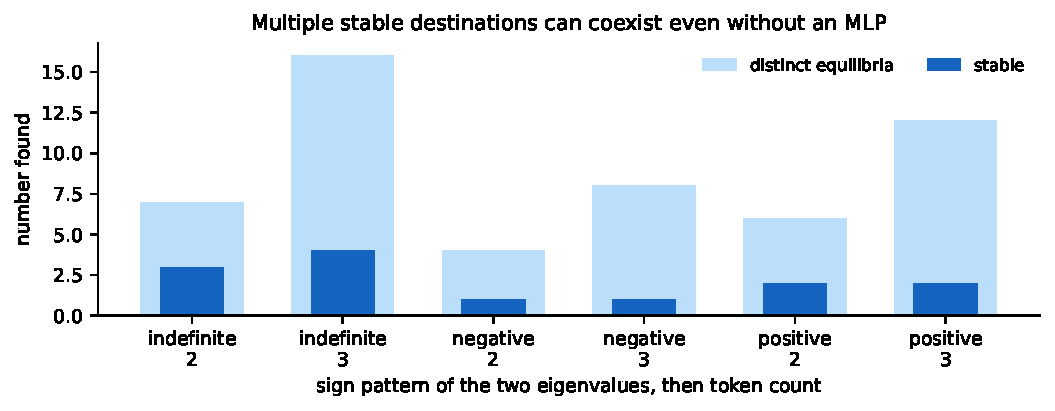
\includegraphics[width=0.92\textwidth]{figures_en/small_equilibrium_catalogue.pdf}
\caption{Catalogue without an MLP for symmetric $V=S$ in dimension two. The spectra
are $(2,-3)$ with $\beta=1.5$, $(-0.4,-4)$ with $\beta=0.03$, and $(3,2)$ with
$\beta=1.5$. The second line of each label is the token count. Numerical search
discovers the branches; theoretical completeness comes from
\eqref{eq:spectral-gram}, not from the number of starts.}
\label{fig:small-catalogue}
\end{figure}

\section{Finite-layer and continuous periodic orbits}
\label{sec:cycles}

\subsection{Finite-layer periodic orbits}

A period-$p$ cycle of the layer is a sequence of $p$ distinct configurations that
returns exactly to its starting point after $p$ applications of \eqref{eq:finite-map}.
This object depends on the layer strength $h$.

\begin{lemma}[A fixed number of layers does not survive unchanged]
\label{lem:fixed-period}
If the layer satisfies $F_h(X)=X+h f(X)+O(h^2)$ and $p$ remains fixed as $h\to0$, then
every limit of a period-$p$ cycle satisfies $f(X)=0$.
\end{lemma}

Indeed, $F_h^p(X)=X+phf(X)+O(h^2)$. A three-layer cycle can therefore collapse to an
equilibrium as layers are weakened. It does not prove the existence of a continuous-time
loop.

\subsection{Continuous periodic orbits}

A continuous cycle is a loop traversed in a time $T>0$. A layer of strength $h$ covers
only a fraction of it, so the number of layers per revolution must grow as $T/h$. This
is the signature measured in \cref{fig:cycle-stability-depth}.

\subsection{Rigid rotations and internal motion}

If all inner products $x_i^{\T}x_j$ remain constant while the entire set rotates, the
shape does not evolve: this is a rigid rotation. In an internal cycle, at least one
inter-token distance changes and then returns. The latter is a stronger phenomenon.

An analytical example already shows that attention without an MLP can rotate. Take one
token on the circle, $S=0$, and
\[
 V=\omega\begin{pmatrix}0&-1\\1&0\end{pmatrix}.
\]
Then $\dot x=Vx$, and the token rotates with period $2\pi/|\omega|$. This rotation is
neutral: it does not show that a loop attracts perturbations. The experiment in
\cref{sec:cycle-experiment} establishes precisely this harder point.

\section{Lyapunov structure of the tied symmetric flow}
\label{sec:no-cycle}

Under $S=V=V^{\T}$ and for $\beta>0$, define
\begin{equation}
 E_\beta(X)=\frac{1}{2\beta}\sum_{i,j=1}^n
 \exp\!\left(\beta x_i^{\T}Vx_j\right).                   \label{eq:energy}
\end{equation}
If $Z_i=\sum_j\exp(\beta x_i^{\T}Vx_j)$, direct calculation gives
\begin{equation}
 \frac{dE_\beta}{dt}=\sum_{i=1}^n Z_i\norm{\dot x_i}^2\geq0.  \label{eq:energy-growth}
\end{equation}
The quantity increases strictly whenever a token moves. A closed trajectory would have
to return to its initial value of $E_\beta$, which is impossible unless it is already
stationary. This is the weighted gradient structure used by Kuehn--Yoon
\cite{kuehnyoon2026spectral}.

At $\beta=0$, the same conclusion holds with
\[
 \Phi(X)=\frac{1}{2n}\left(\sum_i x_i\right)^{\T}
 V\left(\sum_jx_j\right).
\]

The identity uses the full relation $S=V=V^{\T}$, rather than symmetry of $V$ alone.
For independent $S$ and $V$, the calculation does not produce a Lyapunov function.

On the circle at $\beta=0$, the departure from reciprocity is seen exactly in
\begin{equation}
 \frac{\partial\dot\theta_i}{\partial\theta_j}
 -\frac{\partial\dot\theta_j}{\partial\theta_i}
 =\frac1n t_i^{\T}(V-V^{\T})t_j.                          \label{eq:curl}
\end{equation}
The antisymmetric part of $V$ therefore supplies circulation. At $\beta>0$, row-wise
normalization of the weights adds further terms. Even when ordinary cross-derivatives
do not match, the case $S=V=V^{\T}$ remains cycle-free because of the weighted metric
in \eqref{eq:energy-growth}. This detail prevents conflating a Euclidean gradient with
a monotone quantity.

\section{A stable periodic orbit produced by attention alone}
\label{sec:cycle-experiment}

\subsection{Explicit parameters}

The model uses three tokens on the circle, no MLP, and
\begin{equation}
S=\begin{pmatrix}
1.112495&1.768642\\
-2.540753&3.294286
\end{pmatrix},\qquad
V=\begin{pmatrix}
-1.809502&1.419182\\
-1.827949&-3.611608
\end{pmatrix},                                             \label{eq:cycle-matrices}
\end{equation}
with $\beta=1.110063$. The audit measures depth with a scale
$\rho=0.551488$: its equation is
$\dot\theta_i=\rho\sum_j a_{ij}t_i^{\T}Vx_j$. Absorbing $\rho$ into time gives exactly
\eqref{eq:circle}.

This model was isolated by ablating a candidate from a broader search with an MLP.
After all MLP parameters are removed, the cycle persists. Conversely, the MLP alone,
with attention removed, converges to a fixed point. This model-selection step matters:
it establishes existence of an attention cycle, not its frequency under a random
matrix law.

\subsection{Internal geometry along the orbit}

Independent fourth-order Runge--Kutta integration with step $0.005$ gives return time
$T=9.12$ in normalized depth, or $5.030$ in the time of \eqref{eq:circle} after
absorbing $\rho$. The 90th-percentile return residual is
$1.56\times10^{-3}$ radians.

\begin{figure}[ht]
\centering
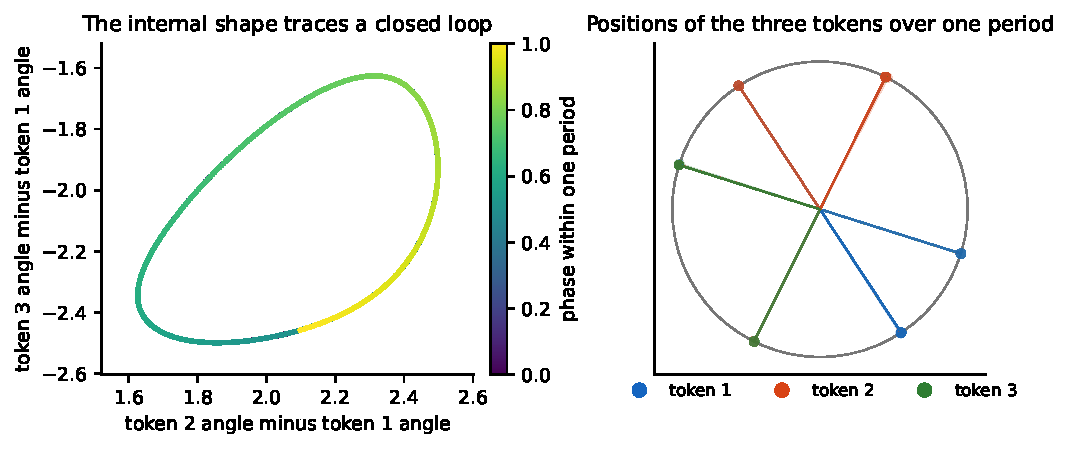
\includegraphics[width=\textwidth]{figures_en/attention_only_cycle_geometry.pdf}
\caption{Internal cycle produced by attention alone. Left: the two relative angles
trace a closed loop; a rigid rotation would be a point. Right: seven phases of one
revolution show the three tokens on the circle. Angles are always taken modulo $2\pi$.}
\label{fig:cycle-geometry}
\end{figure}

All three pairwise inner products vary from $-0.8002$ to $-0.0551$. The shape therefore
changes substantially. The weights sent by token 1 to tokens 1, 2, and 3 respectively
span
\[
[0.298,0.982],\qquad[0.015,0.701],\qquad[0.00018,0.0341].
\]

\begin{figure}[ht]
\centering
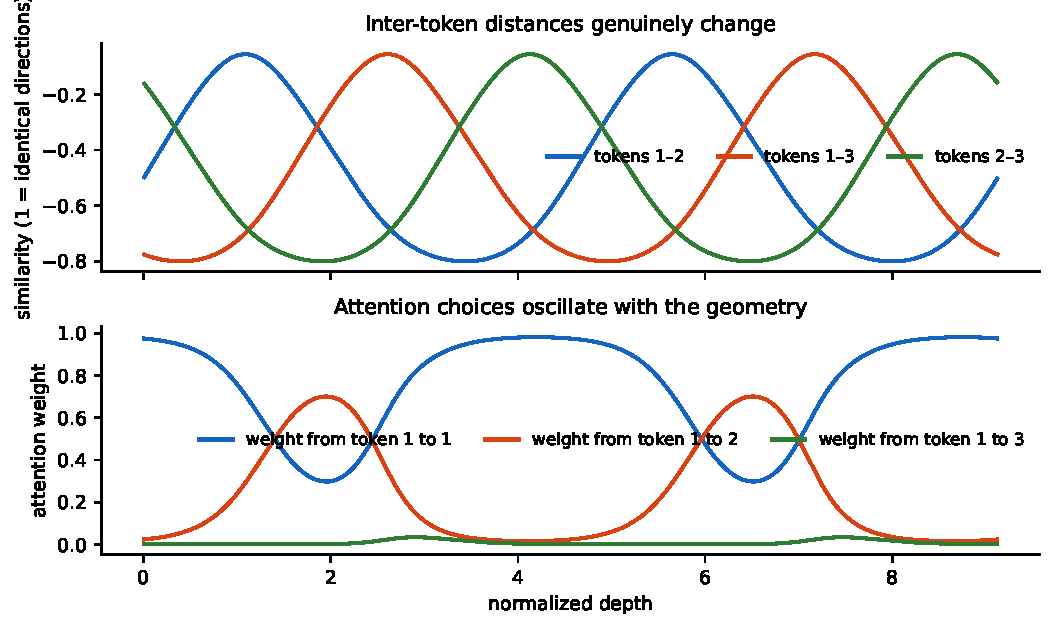
\includegraphics[width=\textwidth]{figures_en/attention_only_cycle_observables.pdf}
\caption{One revolution of the cycle. Top: pairwise token inner products oscillate.
Bottom: the weights in the first attention row oscillate as well. The second period
visible in the distances comes from a role permutation among tokens during the full
return of the labeled angles.}
\label{fig:cycle-observables}
\end{figure}

\subsection{Transverse stability}

On an autonomous closed orbit, a perturbation that merely advances the phase is neither
contracted nor amplified: its theoretical rate is zero. The spectrum measured over
2000 time units is
\begin{equation}
 (-0.00273,\;-0.45676,\;-0.45937).                         \label{eq:cycle-spectrum}
\end{equation}
The first number is the finite approximation to the phase zero. The other two are
clearly negative: deviations transverse to the orbit contract.

We also added 128 Gaussian perturbations with standard deviation $0.08$ around one
point of the cycle. The median distance to the entire orbit decreases from $0.0525$ to
$0.00194$; its 90th percentile decreases from $0.0938$ to $0.00320$. The terminal
plateau is of the same order as the spacing used to store the reference orbit.

\subsection{Scaling of the discrete period with layer strength}
\label{sec:period-scaling}

We replayed the exact layer \eqref{eq:finite-map} at seven ratios, including three
nondyadic values. \Cref{tab:period-scaling} reports the best complete return.

\begin{table}[ht]
\centering
\caption{Return of the attention-only cycle as each layer is weakened. The time per
revolution is the number of layers multiplied by the ratio.}
\label{tab:period-scaling}
\begin{tabular}{@{}rrrr@{}}
\toprule
Ratio & Layers per revolution & Revolution time & Maximum angular error \\
\midrule
$1/16$   & 138  & 8.625 & $2.38\times10^{-2}$ \\
$1/31$   & 275  & 8.871 & $9.46\times10^{-3}$ \\
$1/64$   & 576  & 9.000 & $5.38\times10^{-3}$ \\
$1/127$  & 1151 & 9.063 & $5.43\times10^{-5}$ \\
$1/256$  & 2328 & 9.094 & $1.13\times10^{-3}$ \\
$1/509$  & 4635 & 9.106 & $7.42\times10^{-4}$ \\
$1/1024$ & 9333 & 9.114 & $1.09\times10^{-5}$ \\
\bottomrule
\end{tabular}
\end{table}

The slope of $\log(\text{layers per revolution})$ against
$\log(1/\text{ratio})$ is $1.012$. The revolution time approaches the continuous
equation's period while the layer count diverges.

\begin{figure}[ht]
\centering
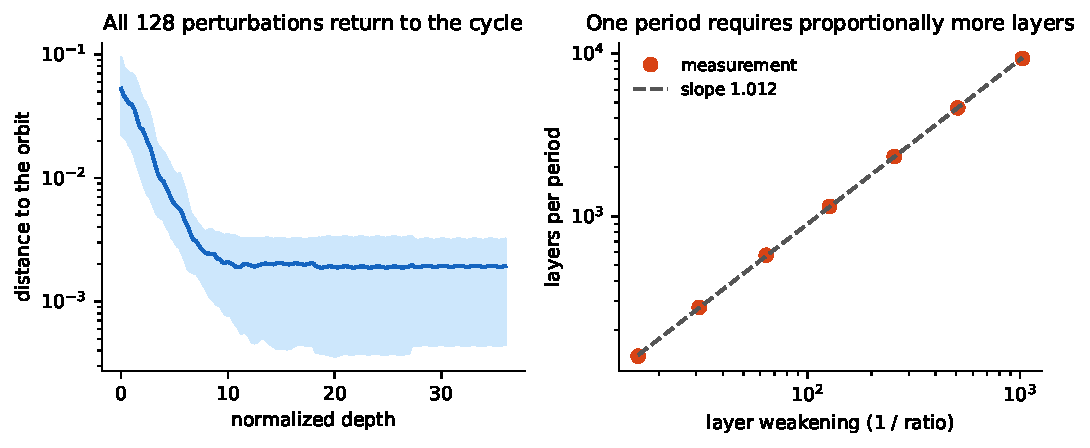
\includegraphics[width=\textwidth]{figures_en/attention_only_cycle_stability_depth.pdf}
\caption{Left: contraction of 128 perturbations toward the orbit. The line is the
median and the band contains 80\% of trials. Right: number of layers per revolution;
the near-unit slope is the signature of a continuous cycle rather than a three- or
four-layer artifact.}
\label{fig:cycle-stability-depth}
\end{figure}

\subsection{Ablations}

\Cref{tab:ablations} prevents an overly broad conclusion. The three most-studied
chaotic candidates do not remain chaotic after the MLP is removed; they converge to an
equilibrium in the attention-only ablation.

\begin{table}[ht]
\centering
\caption{Attention-only ablation results for the representatives studied in detail.}
\label{tab:ablations}
\begin{tabularx}{\textwidth}{@{}lXl@{}}
\toprule
Origin of representative & Attention structure & Result without an MLP \\
\midrule
Three-token cycle, index 1323 & general $S$, general $V$, $\beta>0$ & stable internal cycle \\
Strong three-token chaos, index 2612 & symmetric $S$, general $V$, $\beta>0$ & fixed consensus \\
Weak three-token chaos, index 1051 & $S=V=V^{\T}$, $\beta>0$ & fixed consensus \\
Four-token intermittency, index 3118 & symmetric $S$, general $V$, $\beta=0$ & fixed equilibrium \\
\bottomrule
\end{tabularx}
\end{table}

These tests establish the existence of a stable internal cycle produced by attention
alone. They do not estimate its frequency under random $S,V$. None of the targeted
ablations produced an attention-only chaotic attractor.

\section{Relation to Altafini and Kuehn--Yoon}
\label{sec:comparison}

\subsection{Altafini's assumptions}

Altafini's model does contain the matrices $Q$ and $K$. His main analysis assumes
\begin{equation}
 V=V^{\T},\qquad \lambda_1>0\text{ simple and strictly dominant}.  \label{eq:altafini-assumption}
\end{equation}
It does not assume that $Q^{\T}K$ is symmetric. Under these conditions, Altafini proves
that the zero-output equilibria he calls polygonal are unstable. He also shows that
bipolar consensus and clustering equilibria can be stable and coexist.

\subsection{Compatibility with polygonal instability}

There are three independent reasons:
\begin{enumerate}
  \item the stable triangle in \cref{sec:stability} has nonzero outputs. It belongs to
  Altafini's ``clustering'' class, which his theorem does not declare unstable;
  \item the negative-definite branches of Kuehn--Yoon have no positive eigenvalue and
  therefore fall outside \eqref{eq:altafini-assumption};
  \item the cycle in \eqref{eq:cycle-matrices} uses nonsymmetric $V$ and is not an
  equilibrium. It lies outside both the assumption on $V$ and the question of
  ``stability of a polygonal equilibrium.''
\end{enumerate}

\subsection{Consequences of the Kuehn--Yoon symmetry}

Kuehn--Yoon impose the stronger relation
\[
 Q^{\T}K=V=V^{\T}.
\]
It supplies the monotone quantity \eqref{eq:energy}. Their paper proves global
selection results inside a cone when the dominant positive eigenvalue exceeds all
others in magnitude, and for two tokens when $V$ is negative definite
\cite{kuehnyoon2026spectral}. Our characterization \eqref{eq:spectral-gram} addresses
the different question ``what are all possible stationary points?'', including mixed
branches and multiplicities, without claiming that every one is reached from a generic
initialization.

\begin{table}[ht]
\centering
\caption{Scope of the three analyses.}
\label{tab:scope}
\begin{tabularx}{\textwidth}{@{}lYYY@{}}
\toprule
 & Altafini & Kuehn--Yoon & This report \\
\midrule
MLP & absent & absent & absent \\
Score $S=Q^{\T}K$ & general & equal to $V$ & general, then the case equal to $V$ \\
Value $V$ & symmetric, simple positive top eigenvalue & symmetric, selected spectra & general; complete classification when tied symmetric \\
Equilibria & four classes, thresholds on pure branches & spectral selection and pure-branch stability & necessary and sufficient condition, group reduction, spectral--Gram system \\
Cycles & possible cycle noted when $V$ loses symmetry & excluded by the energy & explicit stable internal cycle without an MLP \\
\bottomrule
\end{tabularx}
\end{table}

\section{Conclusion}

Equation \eqref{eq:final-equilibrium} characterizes every equilibrium for arbitrary
$n,d,S,V$. Under $S=V=V^{\T}$, \eqref{eq:spectral-gram} gives an equivalent
spectral--Gram system and \eqref{eq:energy-growth} excludes nonconstant recurrent
orbits. These statements include stable multi-vertex configurations with nonzero
radial output and are consistent with Altafini's instability theorem for the narrower
zero-output polygonal class.

For untied $S,V$, the matrices in \eqref{eq:cycle-matrices} yield a stable internal
periodic orbit. Its transverse spectrum, perturbation experiment, and discrete-period
scaling establish persistence in the continuous-depth limit. The computation is an
existence result for one parameter set. A probabilistic theory for periodic or chaotic
attention-only dynamics under random matrices remains open.

\appendix

\section{Additional proofs}
\label{app:proofs}

\subsection{Proof of the spectral--Gram theorem}

In an eigenbasis of $V$, write $X=C_1\oplus\cdots\oplus C_s$. Projecting
$RXV=MX$ onto the eigenspace of $\lambda_\alpha^\star$ gives
\[
 (\lambda_\alpha^\star R-M)C_\alpha=0.
\]
Multiplication on the right by $C_\alpha^{\T}$ yields
$(\lambda_\alpha^\star R-M)G_\alpha=0$. The identities for $H$ and the diagonals
follow from the orthogonal decomposition.

Conversely, factor any positive solution as
$G_\alpha=C_\alpha C_\alpha^{\T}$ with at most $m_\alpha$ columns. The image of
$G_\alpha$ is the same as that of $C_\alpha$, so the equation for $G_\alpha$ implies
the equation for $C_\alpha$. Placing these factors in orthogonal eigenspaces
reconstructs $X$ and $RXV=MX$. Two factorizations of the same $G_\alpha$ differ by an
internal rotation of the eigenspace, which proves the statement modulo those rotations.

\subsection{Proof of the classification at \texorpdfstring{$\beta=0$}{beta = 0}}

Under uniform attention, every vector field has the form $P_{x_i}z/n$, where
$z=V\sum_jx_j$. If $z=0$, the configuration is stationary. Otherwise every $x_i$ must
be parallel to $z$, hence $x_i\in\{u,-u\}$ with $u=z/\norm z$. The sum equals $cu$.
Then $z=cVu$ is parallel to $u$, so $u$ is an eigenvector. Since $z\neq0$, both $c$ and
the corresponding eigenvalue are nonzero. The converse is immediate.

\subsection{No zero outputs when \texorpdfstring{$V$}{V} is positive definite}

Under $S=V\succ0$, group the $q$ distinct positions $w_a$. The matrix
\[
 \mathcal R_{ab}=\exp\!\left(\beta
 \ip{V^{1/2}w_a}{V^{1/2}w_b}\right)
\]
is strictly positive definite for distinct points and therefore invertible. The
zero-output condition is
$\mathcal R\Diag(r_1,\ldots,r_q)WV=0$. Since
$\mathcal R$, $\Diag(r_1,\ldots,r_q)$, and $V$ are invertible, this equality would
force $W=0$, contradicting the unit norm of its rows. The multi-vertex equilibria that
remain possible must therefore have nonzero radial output.

\section{Exact Jacobian on the circle}
\label{app:jacobian}

This appendix gives a directly programmable formula. Set
\[
 g_{ij}=t_i^{\T}Vx_j,\qquad s_{ij}=x_i^{\T}Sx_j,\qquad
 f_i=\sum_j a_{ij}g_{ij}.
\]
For angle $\theta_k$,
\begin{align}
 D_k s_{ij}
 &=\mathbf 1_{i=k}\,t_i^{\T}Sx_j
 +\mathbf 1_{j=k}\,x_i^{\T}St_j,\\
 D_k g_{ij}
 &=-\mathbf 1_{i=k}\,x_i^{\T}Vx_j
 +\mathbf 1_{j=k}\,t_i^{\T}Vt_j.
\end{align}
Differentiating the softmax then gives
\begin{equation}
 \boxed{
 J_{ik}=\sum_j a_{ij}\left[
 D_k g_{ij}+\beta g_{ij}
 \left(D_k s_{ij}-\sum_\ell a_{i\ell}D_k s_{i\ell}\right)
 \right].}                                                \label{eq:circle-jacobian}
\end{equation}
At an equilibrium, the real parts of the eigenvalues of $J$ determine stability. For a
finite layer, one directly computes the Jacobian of $F_h$; its eigenvalues must have
modulus below one. For small $h$, a continuous rate $\lambda$ gives a layer multiplier
$1+h\lambda+O(h^2)$.

\section{Unbalanced bipolar split}
\label{app:imbalanced}

Let $n_+$ be the number of $+u$ tokens, $n_-$ the number of $-u$ tokens, and
$r=n_+/n_-$. For an eigenvalue $\lambda_p$, define
\[
 c=\e^{2\beta\lambda_p},\qquad
 \sigma(c,r)=\frac{(c-r)(cr-1)}{r(c^2-1)}.
\]
If $\lambda_p>0$, the split is locally stable exactly when
\[
 \lambda_p>\frac{|\log r|}{2\beta},
 \qquad \lambda_k<\lambda_p\sigma(c,r)\quad(k\neq p).
\]
If $\lambda_p<0$, the condition is
\[
 \lambda_p<-\frac{|\log r|}{2\beta},
 \qquad \lambda_p<\lambda_k<\lambda_p\sigma(c,r)\quad(k\neq p).
\]
For $r=1$, $\sigma=\tanh(\beta\lambda_p)$ and we recover
\eqref{eq:positive-bipolar}--\eqref{eq:negative-bipolar}.

\section{Reproducibility and claim traceability}
\label{app:reproducibility}

The main files are:
\begingroup
\small
\raggedright
\begin{itemize}
  \item \path{experiments/spectral_self_attention/non_mlp_report_experiments_en.py}
  for reintegration, perturbations, the depth test, and the English figures;
  \item \path{data/spectral_self_attention/non_mlp_report_results.json}
  for every number displayed in the cycle section;
  \item \path{data/spectral_self_attention/continuous_ode_f4_p3_cycle_attention_only.json}
  for the initial ablation;
  \item \path{data/spectral_self_attention/continuous_lyapunov_spectrum_f4_p3_cycle_attention_only_relaxed2.json}
  for the long spectrum;
  \item \path{data/spectral_self_attention/equilibria/planar_small_systems.csv}
  and \path{search_saturation.csv} for the small-system catalogue;
  \item \path{experiments/spectral_self_attention/equilibrium_catalogue.py}
  and \path{run_equilibrium_catalogue.py} for equilibrium roots.
\end{itemize}
\endgroup

From the repository root, the command
\begin{verbatim}
uv run python \
  experiments/spectral_self_attention/non_mlp_report_experiments_en.py
\end{verbatim}
recreates the four English figures and the JSON summary. The matrices in
\eqref{eq:cycle-matrices}, random seeds, step sizes, durations, and thresholds are
stored in these files.

\begin{table}[ht]
\centering
\caption{Exact status of the main claims.}
\begin{tabularx}{\textwidth}{@{}lX@{}}
\toprule
Claim & Status \\
\midrule
Condition \eqref{eq:final-equilibrium} & necessary and sufficient algebraic theorem \\
System \eqref{eq:spectral-gram} & theorem, complete modulo eigenspace rotations \\
No cycle when $S=V=V^{\T}$ & exact consequence of \eqref{eq:energy-growth} \\
Displayed stable triangle & numerical root, residual $<1.3\times10^{-15}$, contracting Jacobian \\
General cycle without an MLP & numerical evidence: return, spectrum, perturbations, and depth law \\
Absence of chaos without an MLP & not established; only observed in the targeted ablations \\
Frequency of random cycles & not measured in a dedicated survey \\
\bottomrule
\end{tabularx}
\end{table}

\bibliographystyle{plain}
{\small\bibliography{references}}

\end{document}
